\documentclass[12pt,reqno]{amsart}\usepackage[]{graphicx}\usepackage[]{color}
%% maxwidth is the original width if it is less than linewidth
%% otherwise use linewidth (to make sure the graphics do not exceed the margin)
\makeatletter
\def\maxwidth{ %
  \ifdim\Gin@nat@width>\linewidth
    \linewidth
  \else
    \Gin@nat@width
  \fi
}
\makeatother

\definecolor{fgcolor}{rgb}{0.345, 0.345, 0.345}
\newcommand{\hlnum}[1]{\textcolor[rgb]{0.686,0.059,0.569}{#1}}%
\newcommand{\hlstr}[1]{\textcolor[rgb]{0.192,0.494,0.8}{#1}}%
\newcommand{\hlcom}[1]{\textcolor[rgb]{0.678,0.584,0.686}{\textit{#1}}}%
\newcommand{\hlopt}[1]{\textcolor[rgb]{0,0,0}{#1}}%
\newcommand{\hlstd}[1]{\textcolor[rgb]{0.345,0.345,0.345}{#1}}%
\newcommand{\hlkwa}[1]{\textcolor[rgb]{0.161,0.373,0.58}{\textbf{#1}}}%
\newcommand{\hlkwb}[1]{\textcolor[rgb]{0.69,0.353,0.396}{#1}}%
\newcommand{\hlkwc}[1]{\textcolor[rgb]{0.333,0.667,0.333}{#1}}%
\newcommand{\hlkwd}[1]{\textcolor[rgb]{0.737,0.353,0.396}{\textbf{#1}}}%

\usepackage{framed}
\makeatletter
\newenvironment{kframe}{%
 \def\at@end@of@kframe{}%
 \ifinner\ifhmode%
  \def\at@end@of@kframe{\end{minipage}}%
  \begin{minipage}{\columnwidth}%
 \fi\fi%
 \def\FrameCommand##1{\hskip\@totalleftmargin \hskip-\fboxsep
 \colorbox{shadecolor}{##1}\hskip-\fboxsep
     % There is no \\@totalrightmargin, so:
     \hskip-\linewidth \hskip-\@totalleftmargin \hskip\columnwidth}%
 \MakeFramed {\advance\hsize-\width
   \@totalleftmargin\z@ \linewidth\hsize
   \@setminipage}}%
 {\par\unskip\endMakeFramed%
 \at@end@of@kframe}
\makeatother

\definecolor{shadecolor}{rgb}{.97, .97, .97}
\definecolor{messagecolor}{rgb}{0, 0, 0}
\definecolor{warningcolor}{rgb}{1, 0, 1}
\definecolor{errorcolor}{rgb}{1, 0, 0}
\newenvironment{knitrout}{}{} % an empty environment to be redefined in TeX

\usepackage{alltt}
\usepackage{geometry}                % See geometry.pdf to learn the layout options. There are lots.
\geometry{letterpaper}                   % ... or a4paper or a5paper or ... 
%\geometry{landscape}                % Activate for for rotated page geometry
%\usepackage[parfill]{parskip}    % Activate to begin paragraphs with an empty line rather than an indent
\usepackage{graphicx}
\usepackage{amsfonts}
\usepackage{amsthm}
\usepackage{epstopdf}
\usepackage{hyperref}
\usepackage{enumerate}

%Fix \mathbb
\DeclareFontFamily{U}{futm}{}
\DeclareFontShape{U}{futm}{m}{n}{
  <-> s * [.92] fourier-bb
  }{}
\DeclareSymbolFont{Ufutm}{U}{futm}{m}{n}
\DeclareSymbolFontAlphabet{\mathbb}{Ufutm}

%language packages
\usepackage[utf8]{inputenc}
\usepackage[spanish]{babel}

%color packages
\usepackage{amsmath,color,graphicx}
\definecolor{myred}{rgb}{0.6,0,0} 



%Include definitions
%% Place here your \newcommand's and \renewcommand's. Some examples already included.
%%
\renewcommand{\le}{\leqslant}
\renewcommand{\ge}{\geqslant}
\renewcommand{\emptyset}{\ensuremath{\varnothing}}
\newcommand{\ds}{\displaystyle}
\newcommand{\R}{\ensuremath{\mathbb{R}}}
\newcommand{\Q}{\ensuremath{\mathbb{Q}}}
\newcommand{\Z}{\ensuremath{\mathbb{Z}}}
\newcommand{\N}{\ensuremath{\mathbb{N}}}
\newcommand{\T}{\ensuremath{\mathbb{T}}}
\newcommand{\eps}{\varepsilon}
\newcommand{\closure}[1]{\ensuremath{\overline{#1}}}

%MINE
%\newcommand{\norm}[1]{\left\Vert#1\right\Vert}
%\newcommand{\abs}[1]{\left\vert#1\right\vert}
\newcommand{\set}[1]{\left\{#1\right\}}
\newcommand{\epsi}{\varepsilon}
\newcommand{\To}{\longrightarrow}
\newcommand{\BX}{\mathbf{B}(X)}
\newcommand{\A}{\mathcal{A}}
\newcommand{\St}{\mathcal{S}}
\newcommand{\Par}{\mathcal{P}}
\newcommand{\La}{\mathcal{L}}
\newcommand{\F}{\mathcal{F}}

%LINEAR ALGEBRA
\newcommand{\tr}{\mathrm{tr}}
\newcommand{\sign}{\mathrm{sign}}
\providecommand{\norm}[1]{\lVert#1\rVert}

%PROBABILITY
\newcommand{\Var}{\mathrm{Var}\:}
\newcommand{\Cov}{\mathrm{Cov}\:}
\newcommand{\dis}{\mathrm{d}}

%Numerics
\newcommand{\Fb}{\textbf{F}}

%Theorem Styles
\newtheorem{thm}{Theorem}[section]
\newtheorem{cor}[thm]{Corollary}
\newtheorem{lem}[thm]{Lemma}

\theoremstyle{remark}
\newtheorem{rem}[thm]{Remark}

%Mattias
\newcommand{\mpar}[1]{{\marginpar{\tiny #1}}}
\newcommand{\notto}{\nrightarrow}
\newcommand{\Lloc}{L^1_{\mathrm{loc}}}
\newcommand{\Ito}{It{\^o}\ }
\newcommand{\Itos}{It{\^o}'s\ }
\newcommand{\eg}{e.g.\ }
\newcommand{\ie}{i.e.\ }
\newcommand{\as}{a.s.\ }
\newcommand{\iid}{i.i.d.\ }
\newcommand{\qand}{{\quad\text{and}\quad}}
\newcommand{\qor}{{\quad\text{or}\quad}}
\newcommand{\fixme}{{\begin{center}{\textbf{\huge fixme}}\end{center}}}
\newcommand{\work}{{\begin{center}{\textbf{\huge work}}\end{center}}}
\newcommand{\smilie}{{$:\hspace{-1mm}-\hspace{-0.5mm})$}}
\newcommand{\pa}{{\partial}}

%\newcommand{\acim}{\textsc{acim}\xspace}
%\newcommand{\acims}{\textsc{acim}s\xspace}

%%
%% Place here your \newtheorem's:
%%

%% Some examples commented out below. Create your own or use these...
%%%%%%%%%\swapnumbers % this makes the numbers appear before the statement name.
%\theoremstyle{plain}
%\newtheorem{thm}{Theorem}[chapter]
%\newtheorem{prop}[thm]{Proposition}
%\newtheorem{lemma}[thm]{Lemma}
%\newtheorem{cor}[thm]{Corollary}

%\theoremstyle{definition}
%\newtheorem{define}{Definition}[chapter]

%\theoremstyle{remark}
%\newtheorem*{rmk*}{Remark}
%\newtheorem*{rmks*}{Remarks}

%% This defines the "proo" environment, which is the same as proof, but
%% with "Proof:" instead of "Proof.". I prefer the former.
%\newenvironment{proo}{\begin{proof}[Proof:]}{\end{proof}}


\DeclareGraphicsRule{.tif}{png}{.png}{`convert #1 `dirname #1`/`basename #1 .tif`.png}

\title{Generación de números pseudo-aleatorios.}
\author{Vidal Alcalá.}
%\date{}                                           % Activate to display a given date or no date
\IfFileExists{upquote.sty}{\usepackage{upquote}}{}
\begin{document}

\maketitle

En los modelos de simulación es común encontrarse con variables aleatorias con diversas distribuciones. Los lenguajes de programación vienen con generadores de números pseudo-aleatorios que funcionan bien en general y ofrecen una amplia gama de distribuciones. Sin embargo, de vez en cuando aparecen distribuciones que no están implementadas y se vuelve indispensable saber como crear nuestros propios generadores.

\section{Notación.}
Supongamos que $X$ es una variable aleatoria. La función de distribución de $X$, $F_{X}:\R\to [0,1]$ se define como
\begin{equation}
  \begin{split}
  F_{X}(x) &= P(X\leq x) \:.
	\end{split}
\end{equation}
La función de densidad $f_{X}:\R \to \R $ se define mediante la ecuación
\begin{equation}
  \begin{split}
  P( X\in (a,b) ) &= \int_{a}^{b}f_X(y)\:dy,\qquad a\leq b\:.
  \end{split}
\end{equation}
A menos que lo especifique de otra manera, voy a asumir que las variables aleatorias tienen función de densidad $f_X$ continua.

% Nótese que si tomamos $ a = x, b = x + dx $ con $dx$ pequeño obtenemos
% \begin{equation*}
%   \begin{split}
%   P( X\in (x , x +  dx ) ) &= \int_{x}^{x + dx}f_X(y)\:dy \\
%   \end{split}
% \end{equation*}
% Usando que \emph{$f_{X}$ es una función continua}, el Teorema del valor medio para integrales nos permite calcular
% \begin{equation*}
%   \begin{split}
%   \lim_{dx \to 0} \frac{\int_{x}^{x + dx}f_X(y)\:dy-f_{X}(x) dx }{dx}&=
%   \lim_{dx \to 0} \frac{f_X(\xi) dx-f_{X}(x) dx }{dx},\qquad x<\xi<x+dx\\
%   &= \lim_{dx \to 0} ( f_X(\xi) -f_{X}(x) )\\
%   &= 0 \:.
%   \end{split}
% \end{equation*}
% Hemos probado que la diferencia $P( X\in (x , x +  dx ) ) - f_X(x)\:dx$ converge a zero más rápido dx, lo cual se escribe de la siguiente forma. 
% \begin{equation*}
%   \begin{split}
%   P( X\in (x , x +  dx ) ) - f_X(x)\:dx &= o(dx)\:,
%   \end{split}
% \end{equation*}
% lo cual podemos reescribir como
% \begin{equation*}
%   \begin{split}
%   P( X\in (x , x +  dx ) ) &= f_X(x)\:dx + o(dx)\:.
%   \end{split}
% \end{equation*}



\section{Densidad uniforme en $(0,1)$.}
La variable aleatoria $U$ tiene densidad uniforme en el intervalo $[0,1]$ si
\begin{equation*}
  \begin{split}
	P(U\in [r,s]) &= r - s,\qquad 0< r \leq s < 1 \:.
	\end{split}
\end{equation*}
Se sigue que la probabilidad de que $U$ pertenezca a un intervalo no depende de la posición del intervalo y solo depende de la longitud del intervalo. En términos de funciones de distribución y densidad tenemos
\begin{equation}\label{disUniforme}
  \begin{split}
  F(u) &= P(U \leq u) = \begin{cases}
           0 & u < 0\\
           u & 0\leq u \leq 1\\
           1 & 1 < u
	        \end{cases}
  \end{split}
\end{equation}
\begin{equation}\label{denUniforme}
  \begin{split}
  f(u) &=F'(u)= \begin{cases}
           0 & u < 0\\
           1 & 0\leq u \leq 1\\
           0 & 1 < u\:.
          \end{cases}
  \end{split}
\end{equation}
Escribiremos $X \sim U(0,1)$ para denotar que la variable aleatoria $X$ tiene distribución uniforme en el intervalo $(0,1)$. 

\section{Método de congruencias lineales.}
El objetivo es construir una secuencia $u_{1},u_2,\ldots, u_L$ de números que sean \emph{aproximadamente} aleatorios , independientes e idénticamente distribuidos, con distribución $U(0,1)$. El método de congruencia lineal define una secuencia de \emph{semillas} $s_n$ mediante la iteración
\begin{equation*}
	\begin{split}
	s_{n+1} = (a s_n + c) \text{ mod } m \:.
	\end{split}
\end{equation*}
La siguiente figura muestra la gráfica de la función $s_0\to  (a s_0 + c) \text{ mod } m$ con los parámetros $a =5 , c = 7 , m = 8$.
\begin{knitrout}
\definecolor{shadecolor}{rgb}{0.969, 0.969, 0.969}\color{fgcolor}\begin{kframe}
\begin{alltt}
\hlstd{a} \hlkwb{<-} \hlnum{20}
\hlstd{c} \hlkwb{<-} \hlnum{7}
\hlstd{m} \hlkwb{<-} \hlnum{8}
\hlcom{# definir funcion x (mod m) para x,y > 0}
\hlstd{mod} \hlkwb{<-} \hlkwa{function}\hlstd{(}\hlkwc{x}\hlstd{,} \hlkwc{m}\hlstd{) \{}
    \hlstd{((x}\hlopt{/}\hlstd{m)} \hlopt{-} \hlkwd{floor}\hlstd{(x}\hlopt{/}\hlstd{m))} \hlopt{*} \hlstd{m}
\hlstd{\}}

\hlstd{s0} \hlkwb{<-} \hlkwd{seq}\hlstd{(}\hlnum{0}\hlstd{, m,} \hlnum{0.001}\hlstd{)}
\hlstd{s1} \hlkwb{<-} \hlkwd{mod}\hlstd{(a} \hlopt{*} \hlstd{s0} \hlopt{+} \hlstd{c, m)}
\end{alltt}
\end{kframe}
\end{knitrout}

\begin{knitrout}
\definecolor{shadecolor}{rgb}{0.969, 0.969, 0.969}\color{fgcolor}\begin{kframe}
\begin{alltt}
\hlkwd{plot}\hlstd{( s0 , s1 )}
\end{alltt}
\end{kframe}
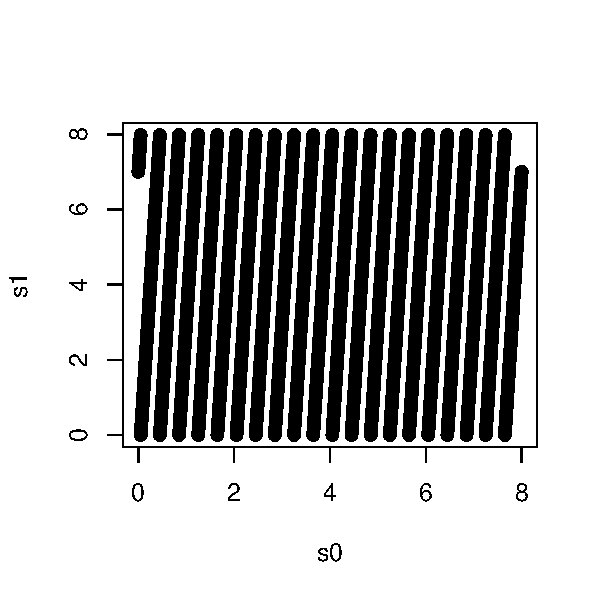
\includegraphics[width=.45\linewidth]{figure/iteracion2_} 

\end{knitrout}

La secuencia de semillas $s_n$ define la secuencia $u_n$ mediante la ecuación $u_n = s_n / m$. Es claro que la secuencia $u_n$ no es aleatoria, es \emph{pseudo-aleatoria}. Sin embargo, para el propósito de simulaciones tipo Monte Carlo, la propiedad que debe satisfacer es que
\begin{equation}\label{MonteCarlo}
  \begin{split}
	\frac{1}{L}\sum_{n=1}^{L} f(u_n) \sim E[f(U)]\:,
	\end{split}
\end{equation}
para $L$ grande donde $U$ es una variable aleatoria con distribución normal y $f$ es una función continua en el intervalo $[0,1]$.

Cualquier generador de este tipo tiene solo $m$ posible valores para las semillas $s_n$ y por lo tanto la secuencia $s_n$ se cicla en $m$ o menos iteraciones y por lo tanto no es razonable esperar que la ecuación \eqref{MonteCarlo} se cumpla para $L > m$. El generador \emph{Learmouth-Lewis} usa $a = 7^5$ y $ m = 2^{31}-1$ y generadores mas sofisticados usan $ m \sim 2^{128}\sim 10^{38} $. El generador Mersenne-Twister , utilizado en la rutina \verb+ runif()+ de R, se cicla después de $2^{19937}\sim 10^{6001}$ iteraciones y es el preferido en aplicaciones.

Un método importante en aplicaciones es la habilidad de ajustar la semilla del generador. Esto permite reproducir resultados como se hace en el siguiente ejemplo.
\begin{knitrout}
\definecolor{shadecolor}{rgb}{0.969, 0.969, 0.969}\color{fgcolor}\begin{kframe}
\begin{alltt}
\hlkwd{set.seed}\hlstd{(}\hlnum{1001}\hlstd{)}
\hlcom{## salva la semilla actual}
\hlkwd{save}\hlstd{(}\hlstr{".Random.seed"}\hlstd{,} \hlkwc{file} \hlstd{=} \hlstr{"random_state_seed1001.RData"}\hlstd{)}
\hlkwd{runif}\hlstd{(}\hlnum{1}\hlstd{)}
\end{alltt}
\begin{verbatim}
## [1] 0.9857
\end{verbatim}
\begin{alltt}
\hlkwd{runif}\hlstd{(}\hlnum{1}\hlstd{)}
\end{alltt}
\begin{verbatim}
## [1] 0.4126
\end{verbatim}
\begin{alltt}
\hlkwd{runif}\hlstd{(}\hlnum{1}\hlstd{)}
\end{alltt}
\begin{verbatim}
## [1] 0.4295
\end{verbatim}
\begin{alltt}
\hlcom{## Restaurar la semilla después de set.seed()}
\hlkwd{load}\hlstd{(}\hlstr{"random_state_seed1001.RData"}\hlstd{)}
\hlkwd{runif}\hlstd{(}\hlnum{1}\hlstd{)}
\end{alltt}
\begin{verbatim}
## [1] 0.9857
\end{verbatim}
\end{kframe}
\end{knitrout}

También es posible continuar una simulación que ha sido interrumpida si salvamos la semilla después de cada cierto número de iteraciones y reiniciamos la simulación con la última semilla guardada.

\section{Método de la transformada inversa.}
El objetivo es generar muestras de una variable aleatoria $X$ a partir de una variable aleatoria uniforme $U$. En realidad es más fácil generar una variable uniforme a partir de $X$ y su función de distribución $F_{X}$. Simplemente define $U = F_X(X)$. Asumiendo que $F_{X}:\R\to (0,1)$ es continua y estrictamente creciente podemos calcular para $0<u<1$
\begin{equation}\label{ideaPrincipal}
  \begin{split}
   P[F_X(X)\leq u ] &= P[X\leq F_X^{-1}(u)]\\
   &= F_X(F_X^{-1}(u))\\
   &= u\:.
  \end{split}
\end{equation}
Este cálculo muestra que $F_X(X)$ tiene función de distribución uniforme (ver ecuación \eqref{disUniforme}).El siguiente Teorema nos da condiciones suficientes para ejecutar el procedimiento inverso en los casos de interés en aplicaciones.
\begin{thm}
Supongamos que $F_{X}$ es la función de distribución de la variable aleatoria $X$ con valores en un intervalo $I=(a,b)$ (no excluimos la posibilidad $a = -\infty$ o $b = +\infty$) y que $F_{X}:\R \to (0,1)$ es estrictamente creciente y continua en el intervalo $I$. Entonces existe la inversa por la derecha $F_{X}^{-1}:(0,1)\to I$ y esta inversa es una función estrictamente creciente. Esto quiere decir que para cada $u\in (0,1)$ tenemos
\begin{equation}\label{distribucionInversa}
  \begin{split}
  F_{X}(F_{X}^{-1}(u)) = u  , \qquad 0 < u < 1\:,\\
  \end{split}
\end{equation}
y además $0 < u_1 \leq u_2 < 1$ si y solo si $F_{X}^{-1}(u_1) \leq F_{X}^{-1}(u_2)$.
\end{thm}
Bajo las hipótesis del Teorema anterior tenemos que $F_{X}^{-1}(U)\leq x$ y $F_{X}(F_{X}^{-1}(U))\leq F_{X}(x)$ son el mismo evento y por lo tanto
\begin{equation}\label{DistribucionInversa}
  \begin{split}
  P[F_{X}^{-1}(U)\leq x] &= P[F_{X}(F_{X}^{-1})(U)\leq F_{X}(x)]\\ 
  &= P[U \leq F_X(x) ]\\
  &= F_X (x)\:.
  \end{split}
\end{equation}
Se sigue que la variable aleatoria $F_{X}^{-1}(U)$ tiene función de distribución $F_X$. Cuando sea claro cuál es la variable aleatoria $X$ en cuestión, escribiremos $F$ en lugar de $F_X$.

La discusión anterior sugiere el siguiente algoritmo para generar $L$ muestras independientes de una variable aleatoria $X$ con función de distribución $F(x)$, denotadas por $x_1,x_2,\ldots, x_L$.
\begin{enumerate}
\item Genera $L$ muestras aleatorias i.i.d $u_{n}\sim U[0,1]$.
\item Encuentra las soluciones $x_n$ de las ecuaciones $F(x_n)=u_n$ (equivalente a $x_n = F^{-1}(u_n)$).
\end{enumerate}
Por supuesto, las muestras $x_n$ son independientes ya que las muestras uniformes $u_n$ lo son. El segundo paso del algoritmo se resuelve de manera analítica en la mayoría de las aplicaciones. Ilustraremos la metodología con un ejemplo.

La distribución exponencial con parámetro $\lambda>0$ tiene función de densidad $f(x) = \lambda e^{-\lambda x}$ para $x>0$ y función de distribución
\begin{equation}\label{distribucionExp}
  \begin{split}
  F(x) &= 1-e^{-\lambda x}\:.
  \end{split}
\end{equation}
Es común modelar tiempos de espera con la distribución exponencial. La media de la distribución es $\frac{1}{\lambda}$ y la varianza es $\frac{1}{\lambda^2}$. 

Primero escribimos $x$ en función de $u$ usando la ecuación $F(x) = u$.
\begin{equation*}
  \begin{split}
  1-e^{-\lambda x} &= u \\
  1-u &= e^{-\lambda x} \\
  \log(1-u) &= -\lambda x\\
  -\frac{\log(1-u)}{\lambda} &= x\\
  \end{split}
\end{equation*}
Entonces, hemos obtenido que $F^{-1}(u) = -\frac{\log(1-u)}{\lambda} $. Ahora generamos $L$ muestras uniformes y las transformamos usando $F^{-1}(u)$.
\begin{knitrout}
\definecolor{shadecolor}{rgb}{0.969, 0.969, 0.969}\color{fgcolor}\begin{kframe}
\begin{alltt}
\hlcom{## parametros}
\hlstd{L} \hlkwb{=} \hlnum{1e+05}
\hlstd{lambda} \hlkwb{<-} \hlnum{2}
\hlstd{u} \hlkwb{<-} \hlkwd{runif}\hlstd{(L)}
\hlstd{x} \hlkwb{<-} \hlopt{-}\hlstd{(}\hlnum{1}\hlopt{/}\hlstd{lambda)} \hlopt{*} \hlkwd{log}\hlstd{(}\hlnum{1} \hlopt{-} \hlstd{u)}
\end{alltt}
\end{kframe}
\end{knitrout}

Finalmente comparamos el histograma de las muestras $x_n$ con la densidad exponencial $f(x) = \lambda e^{-\lambda x}$.
\begin{knitrout}
\definecolor{shadecolor}{rgb}{0.969, 0.969, 0.969}\color{fgcolor}\begin{kframe}
\begin{alltt}
\hlstd{xHist} \hlkwb{<-} \hlkwd{hist}\hlstd{(x,} \hlkwc{prob} \hlstd{=} \hlnum{TRUE} \hlstd{,} \hlkwc{breaks} \hlstd{=} \hlnum{10}\hlopt{*}\hlkwd{log}\hlstd{(L))}
\hlkwd{curve}\hlstd{( lambda}\hlopt{*}\hlkwd{exp}\hlstd{(}\hlopt{-}\hlstd{lambda}\hlopt{*}\hlstd{x), xHist}\hlopt{$}\hlstd{mids[}\hlnum{1}\hlstd{] , xHist}\hlopt{$}\hlstd{mids[}\hlkwd{length}\hlstd{(xHist}\hlopt{$}\hlstd{mids)] ,}
       \hlkwc{add} \hlstd{=} \hlnum{TRUE}\hlstd{,} \hlkwc{col} \hlstd{=} \hlstr{'red'}\hlstd{)}
\end{alltt}
\end{kframe}
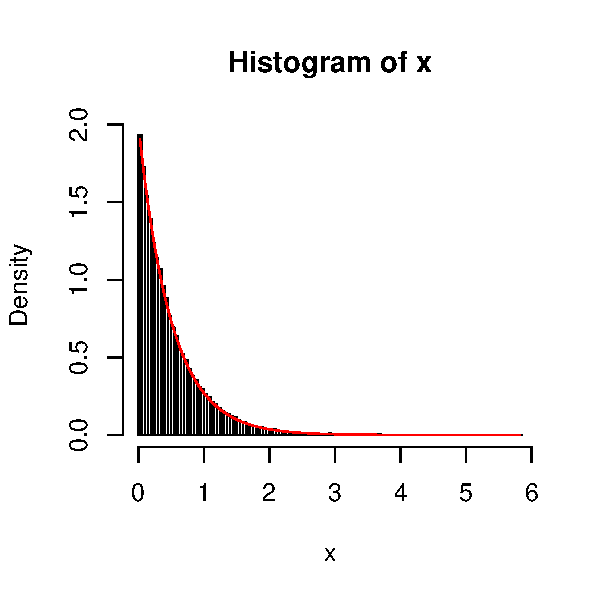
\includegraphics[width=.60\linewidth]{figure/hist_} 

\end{knitrout}


El método de la transformación inversa se puede aplicar también entre dos
variables aleatorias $X,Y$ relacionadas mediante $Y = G(X)$. Aquí necesitamos asumir que la función $G$ es diferenciable y $G'(x)\neq 0$ para cada valor $x$ que pueda tomar $X$. En este caso tenemos
\begin{equation}\label{cambioVariable}
  \begin{split}
  f_{Y}(y) &= \pm \frac{f_{X}(G^{-1}(y))}{G'(G^{-1}(y))}\:.
  \end{split}
\end{equation}
En realidad, es más fácil explicar la metodología en un cambio de variable en particular en lugar de usar la fórmula anterior. El siguiente ejemplo ilustra el procedimiento. Supongamos que $X$ es una v.a. exponencial con parámetro $\lambda$ y $ Y = X^2$.
\begin{enumerate}
\item Escribir la función de densidad de $X$ en \emph{notacion} diferencial.
\begin{equation}\label{density_x}
  \begin{split}
  f_{X}(x) dx &= \lambda e^{-\lambda x} dx,\qquad x > 0\:.
  \end{split}
\end{equation}
\item Sustituir $x$ y $dx$ en la ecuación anterior usando la relación $y = x^2$. 
Despejando $x$ obtenemos
\begin{equation}\label{x}
  \begin{split}
  x &= \sqrt{y} x > 0\:,  
  \end{split}
\end{equation}
y calculando la diferencial el resultado es
\begin{equation}\label{dx}
  \begin{split}
  dy &= d(x^2) = 2\:x\:dx\\
  \frac{dy}{2\:x} &= dx \\
  \frac{dy}{2\sqrt{y}} &= dx
  \end{split}
\end{equation}
Finalmente sustituimos \eqref{x} y \eqref{dx} en la ecuación \eqref{density_x} para obtener
\begin{equation}\label{substitute_y}
  \begin{split}
  f_{X}(x) dx &= \lambda \frac{e^{-\lambda \sqrt{y}}}{2\sqrt{y}}dy,\qquad y > 0\:.
  \end{split}
\end{equation}
\item El factor enfrente del diferencial $dy$ es la función de densidad de la variable aleatoria $Y$, en otras palabras
\begin{equation}\label{density_y}
  \begin{split}
  f_{Y}(y) &= \lambda \frac{e^{-\lambda \sqrt{y}}}{2\sqrt{y}},\qquad y > 0\:.
  \end{split}
\end{equation}

\end{enumerate}
\section{Ejercicios}
\begin{enumerate}
\item Genera 10,000 muestras independientes de la variable aleatoria $X$ con función de densidad
\begin{equation}\label{ejercicio1}
  \begin{split}
  f(x) &= \frac{1}{4}(x+1)^3,\qquad -1 < x < 1\:.
  \end{split}
\end{equation}
Compara el histograma de tus muestras con la función de densidad \eqref{ejercicio1} para comprobar que tus muestras tienen la distribución correcta.
\item Considera una variable aleatoria $T$ con función densidad
\begin{equation}\label{stopTime}
  \begin{split}
  f(t) &= \frac{1}{\sqrt{2\pi t^3}} e^{-1/2t},\qquad t>0\:.
  \end{split}
\end{equation}
\begin{enumerate}
\item Calcula la función de densidad de $X=\frac{1}{\sqrt{T}}$.
\item Genera 10,000 muestras independientes de $T$ usando la función \verb+ rnorm()+ y una transformación inversa. Compara el histograma de tus muestras con la función de densidad \eqref{stopTime} para comprobar que tus muestras tienen la distribución correcta.
\end{enumerate}

\item Genera 10,000 muestras independientes de la variable aleatoria $X$ con función de densidad
\begin{equation}\label{ejercicio3}
  \begin{split}
  f(x) &= x e^{-x^2/2}, \qquad x > 0\:.
  \end{split}
\end{equation}
Compara el histograma de tus muestras con la función de densidad \eqref{ejercicio1} para comprobar que tus muestras tienen la distribución correcta.

\end{enumerate}

\section{Método de aceptación-rechazo.}
Cuando no es posible calcular la función de distribución $F$ de una variable aleatoria $X$, debemos utilizar otros métodos que no dependan de la integración de la función de densidad $f$. El método de aceptación-rechazo utiliza muestras de una v.a. $Y$ para generar muestras de $X$. La idea es transformar las probabilidades de que la v.a. tome un valor en lugar de transformar los valores mismos. Supongamos que tenemos una función $p:\R\to(0,1]$ la cual llamaremos la \emph{probabilidad de aceptación}. Ahora supongamos que las muestras de $X$ se generan a partir de muestras de $Y$ con el siguiente algoritmo.
\begin{enumerate}
\item Genera una muestra $Y_{1}$ de la v.a. $Y$.
\item Con probabilidad $p(Y_{1})$ declara que la muestra de X es $\overline{X}=Y_{1}$ y con probabilidad $1-p(Y_{1})$ regresa al paso (1).
\end{enumerate}
Podemos calcular la función de densidad de la v.a. que se ha generado con el algoritmo anterior de la siguiente forma. Denotamos por $N$ el paso en el que se acepta la muestra de la v.a. $Y$.
\begin{equation}
  \begin{split}
  P(\overline{X} = x )
  &=\sum_{n=1}^{\infty} P( Y_n =x , N = n , N > (n-1) )\\
  &=\sum_{n=1}^{\infty} P( N = n | Y_n = x , N >(n-1) ) P( Y_n = x , N >(n-1) )\\
  &= \sum_{n=1}^{\infty} P( N = n | Y_n = x , N >(n-1) ) P( Y_n = x ) P (N >(n-1))\\
  &= p(x) f_{Y}(x) \sum_{n=1}^{\infty} P (N >(n-1))\\
  &= p(x) f_{Y}(x) \sum_{n=1}^{\infty} P(N >(n-1))\:.
  \end{split}
\end{equation}
% INTEGRAL NOTATION
% \begin{equation}\label{aceptacionRechazo}
%   \begin{split}
%   P(\overline{X}\in (x,x +dx))
%   &=\sum_{n=1}^{\infty} P( Y_n \in (x,x + dx) , N = n , N > (n-1) )\\
%   &=\sum_{n=1}^{\infty} P( N = n | Y_n\in x +dx , N >(n-1) ) P( Y_n\in x +dx , N >(n-1) )\\
%   &= \sum_{n=1}^{\infty} P( N = n | Y_n\in x +dx , N >(n-1) ) P( Y_n\in x +dx ) P (N >(n-1))\\
%   &= (p(x) + p'(x)dx + o(dx)) (f_{Y}(x)dx+o(dx)) \sum_{n=1}^{\infty} P (N >(n-1))\\
%   &= p(x) f_{Y}(x) P(N >(n-1)) dx+o(dx)\:.
%   \end{split}
% \end{equation}
Es un ejercicio de probabilidad el mostrar que
\begin{equation}\label{aceptacionRechazo}
  \begin{split}
  \sum_{n=1}^{\infty} P(N >(n-1))&=E[N]\:.
  \end{split}
\end{equation}
Por lo tanto hemos obtenido que la función de densidad de $\overline{X}$ satisface
\begin{equation}\label{aceptacionRechazo}
  \begin{split}
  f_{\overline{X}}(x)
  &=\frac{1}{Z} p(x) f_{Y}(x) \:,
  \end{split}
\end{equation}
con $Z$ una constante. Para que $f_{\overline{X}}(x)$ integre a 1 debemos tener
\begin{equation}\label{partitionConstant1}
  \begin{split}
  Z = \int_{-\infty}^{\infty} p(y) f_{Y}(y) dy\:,
  \end{split}
\end{equation}
y de acuerdo a el cálculo anterior también podemos asegurar que 
\begin{equation}\label{partitionConstant2}
  \begin{split}
  Z = \frac{1}{E[N]}\:.
  \end{split}
\end{equation}
De cualquier forma, no es necesario calcular la constante $Z$ para implementar el método de aceptación-rechazo.

Nuestro objetivo es obtener muestras de una variable aleatoria con función de distribución $f_{X}$ y por lo tanto debemos escoger $p(x)$ tal que
\begin{equation}
  \begin{split}
  f_{X}(x) = \frac{1}{Z} p(x) f_{Y}(x)\\
  p(x) = \frac{1}{Z} \frac{f_{X}(x)}{f_{Y}(x)}\:.
  \end{split}
\end{equation}
La ecuación anterior solo tiene sentido si
\begin{equation}\label{absContinuous}
  \begin{split}
   0 \leq \frac{f_{X}(x)}{f_{Y}(x)} < +\infty\:,
  \end{split}
\end{equation}
o en otras palabras, si $f_{X}(x)=0$ cuando $f_{Y}(x)=0$. Cuando la condición \eqref{absContinuous} se cumple, decimos que \emph{$X$ es absolutamente continua con respecto a $Y$}. Para que el método de aceptación rechazo funcione hay que asumir una condición aún más fuerte. Vamos a suponer que existe una constante $M$ tal que
\begin{equation}\label{bounded}
  \begin{split}
   0 \leq \frac{f_{X}(x)}{f_{Y}(x)} < M \:.
  \end{split}
\end{equation}


Ilustraremos la metodología con un ejemplo. Supongamos que queremos generar 10,000 muestras de la v.a. normal $X$ con densidad
\begin{equation}
  \begin{split}
   f_{X}(x) &\propto e^{-x^2/2},\qquad x>0\:,
  \end{split}
\end{equation}
usando muestras de la v.a. exponencial $Y$ con densidad
\begin{equation}\label{absContinuous}
  \begin{split}
   f_{Y}(x) &\propto e^{-x},\qquad  x>0\:,
  \end{split}
\end{equation}
\begin{knitrout}
\definecolor{shadecolor}{rgb}{0.969, 0.969, 0.969}\color{fgcolor}\begin{kframe}
\begin{alltt}
\hlcom{## Limpiar variables}
\hlkwd{rm}\hlstd{(}\hlkwc{list} \hlstd{=} \hlkwd{ls}\hlstd{())}

\hlcom{## parametros}
\hlstd{L} \hlkwb{<-} \hlnum{10000}
\end{alltt}
\end{kframe}
\end{knitrout}


El primer paso es verificar si la condición \eqref{bounded} se cumple.
\begin{equation*}
  \begin{split}
  \frac{ f_{X}(x) }{ f_{Y}(x) } &= \frac{e^{-x^2/2}}{e^{-x}} \\
  &= e^{x-x^2/2}\\
  &\leq e^{1/2}\\
  \end{split}
\end{equation*}
\begin{knitrout}
\definecolor{shadecolor}{rgb}{0.969, 0.969, 0.969}\color{fgcolor}\begin{kframe}
\begin{alltt}
\hlcom{## cota superior}
\hlstd{M} \hlkwb{<-} \hlkwd{exp}\hlstd{(}\hlnum{1}\hlopt{/}\hlnum{2}\hlstd{)}
\end{alltt}
\end{kframe}
\end{knitrout}


El segundo paso es escoger $p(x)$ proporcional a $\frac{f_{X}(x)}{f_{Y}(x)}$, esto es
\begin{equation*}
  \begin{split}
  p(x) &\propto e^{x-x^2/2}\:.
  \end{split}
\end{equation*}
La mayor constante que podemos elegir en la relación de proporcionalidad anterior , manteniendo el requerimiento $p(x) < 1$ para $x>0$ es $e^{-1/2}$. Por lo tanto escogemos
\begin{equation*}
  \begin{split}
   p(x) &=\frac{1}{e^{1/2}} e^{x-x^2/2}\:.
  \end{split}
\end{equation*}
Tiene sentido hacer $p(x)$ lo más grande posible ya que esto aumenta la probabilidad de que las muestras de $Y$ sean aceptadas y por lo tanto se reduce el número de pasos $N$ en el algoritmo de aceptación-rechazo.
\begin{knitrout}
\definecolor{shadecolor}{rgb}{0.969, 0.969, 0.969}\color{fgcolor}\begin{kframe}
\begin{alltt}
\hlcom{## definir p(x)}
\hlstd{p} \hlkwb{<-} \hlkwa{function}\hlstd{(}\hlkwc{x}\hlstd{) \{}
    \hlkwd{return}\hlstd{((}\hlnum{1}\hlopt{/}\hlstd{M)} \hlopt{*} \hlkwd{exp}\hlstd{(x} \hlopt{-} \hlstd{x} \hlopt{*} \hlstd{x}\hlopt{/}\hlnum{2}\hlstd{))}
\hlstd{\}}
\end{alltt}
\end{kframe}
\end{knitrout}

Finalmente, generamos las muestras de $X$ usando el método de aceptación-rechazo.
\begin{knitrout}
\definecolor{shadecolor}{rgb}{0.969, 0.969, 0.969}\color{fgcolor}\begin{kframe}
\begin{alltt}
\hlcom{## Generar L muestras de X}
\hlstd{x} \hlkwb{<-} \hlkwd{c}\hlstd{()}
\hlstd{y} \hlkwb{<-} \hlkwd{c}\hlstd{()}
\hlkwa{for} \hlstd{(i} \hlkwa{in} \hlnum{1}\hlopt{:}\hlstd{L) \{}
    \hlstd{y} \hlkwb{<-} \hlkwd{rexp}\hlstd{(}\hlnum{1}\hlstd{)}
    \hlstd{pAceptar} \hlkwb{<-} \hlkwd{p}\hlstd{(y)}
    \hlstd{pAceptar}
    \hlstd{u} \hlkwb{<-} \hlkwd{runif}\hlstd{(}\hlnum{1}\hlstd{)}
    \hlkwa{while} \hlstd{(u} \hlopt{>} \hlstd{pAceptar) \{}
        \hlstd{y} \hlkwb{<-} \hlkwd{rexp}\hlstd{(}\hlnum{1}\hlstd{)}
        \hlstd{pAceptar} \hlkwb{<-} \hlkwd{p}\hlstd{(y)}
        \hlstd{u} \hlkwb{<-} \hlkwd{runif}\hlstd{(}\hlnum{1}\hlstd{)}
    \hlstd{\}}
    \hlstd{x[i]} \hlkwb{<-} \hlstd{y}
    \hlstd{x}
\hlstd{\}}
\end{alltt}
\end{kframe}
\end{knitrout}

Verificamos que el método es correcto.
\begin{knitrout}
\definecolor{shadecolor}{rgb}{0.969, 0.969, 0.969}\color{fgcolor}\begin{kframe}
\begin{alltt}
\hlcom{# El histograma para las muestras de X}
\hlstd{xHist} \hlkwb{<-} \hlkwd{hist}\hlstd{(x,} \hlkwc{prob} \hlstd{=} \hlnum{TRUE} \hlstd{,} \hlkwc{breaks} \hlstd{=} \hlnum{10}\hlopt{*}\hlkwd{log}\hlstd{(L))}

\hlcom{# La densidad de X}
\hlkwd{curve}\hlstd{(} \hlnum{2.0}\hlopt{*}\hlkwd{dnorm}\hlstd{(x), xHist}\hlopt{$}\hlstd{mids[}\hlnum{1}\hlstd{] , xHist}\hlopt{$}\hlstd{mids[}\hlkwd{length}\hlstd{(xHist}\hlopt{$}\hlstd{mids)] ,}
       \hlkwc{add} \hlstd{=} \hlnum{TRUE}\hlstd{,} \hlkwc{col} \hlstd{=} \hlstr{'red'}\hlstd{)}
\end{alltt}
\end{kframe}
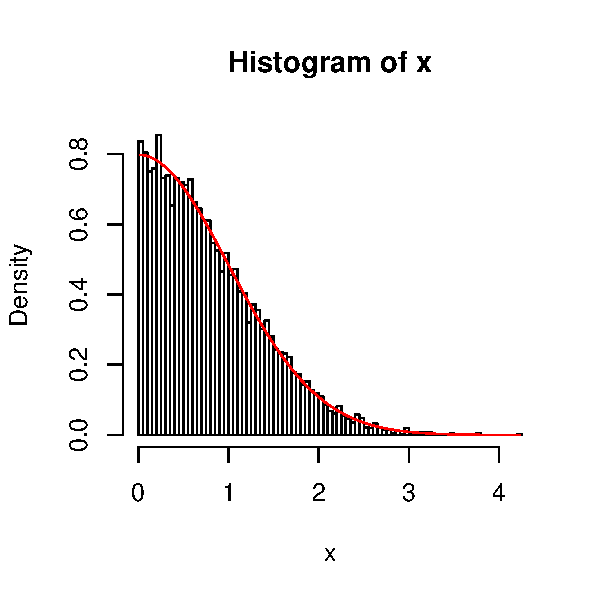
\includegraphics[width=.60\linewidth]{figure/histRejection_1} 
\begin{kframe}\begin{alltt}
\hlcom{#crear una nueva figura}
\hlkwd{plot.new}\hlstd{()}

\hlcom{# La densidad de Y}
 \hlkwd{curve}\hlstd{(} \hlkwd{exp}\hlstd{(}\hlopt{-}\hlstd{x), xHist}\hlopt{$}\hlstd{mids[}\hlnum{1}\hlstd{] , xHist}\hlopt{$}\hlstd{mids[}\hlkwd{length}\hlstd{(xHist}\hlopt{$}\hlstd{mids)] ,} \hlkwc{col} \hlstd{=} \hlstr{'green'}\hlstd{)}

\hlcom{# La densidad de X}
\hlkwd{curve}\hlstd{(} \hlnum{2.0}\hlopt{*}\hlkwd{dnorm}\hlstd{(x), xHist}\hlopt{$}\hlstd{mids[}\hlnum{1}\hlstd{] , xHist}\hlopt{$}\hlstd{mids[}\hlkwd{length}\hlstd{(xHist}\hlopt{$}\hlstd{mids)] ,} \hlkwc{add} \hlstd{=} \hlnum{TRUE} \hlstd{,} \hlkwc{col} \hlstd{=} \hlstr{'red'}\hlstd{)}

\hlcom{# La probabilidad de aceptación}
\hlkwd{curve}\hlstd{(} \hlkwd{p}\hlstd{(x), xHist}\hlopt{$}\hlstd{mids[}\hlnum{1}\hlstd{] , xHist}\hlopt{$}\hlstd{mids[}\hlkwd{length}\hlstd{(xHist}\hlopt{$}\hlstd{mids)] ,}
       \hlkwc{add} \hlstd{=} \hlnum{TRUE}\hlstd{,} \hlkwc{col} \hlstd{=} \hlstr{'blue'}\hlstd{)}
\end{alltt}
\end{kframe}
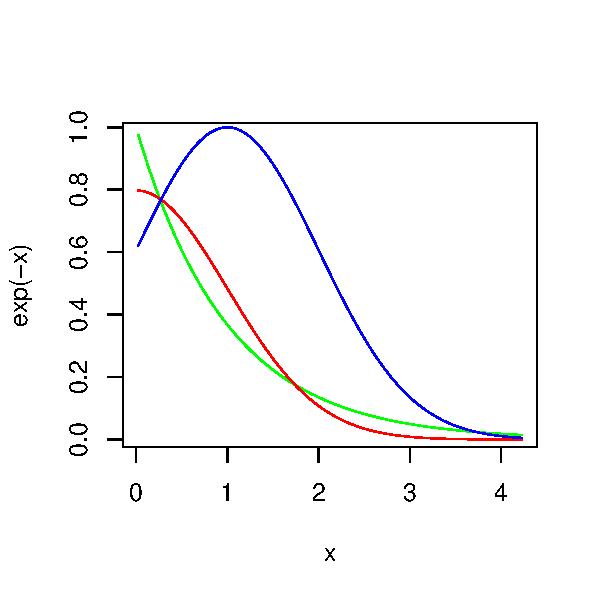
\includegraphics[width=.60\linewidth]{figure/histRejection_2} 

\end{knitrout}


\section{Ejercicios.}
Genera 10,000 muestras de la variable aleatoria $X$ con función de densidad
\begin{equation*}
  \begin{split}
   f_{X}(x) &\propto (x-\mu)\exp\biggl(\frac{-x^2}{2}\biggr),\qquad x>\mu>0\:,
  \end{split}
\end{equation*}
usando el método de aceptación rechazo con muestras de la variable aleatoria $Y$ con función de densidad
\begin{equation*}
  \begin{split}
   f_{Y}(y) = y\:\exp\biggl(\frac{-y^2}{2}\biggr),\qquad y>0 \:.
  \end{split}
\end{equation*}


\end{document}
